\documentclass[american,]{article}
\usepackage{lmodern}
\usepackage{amssymb,amsmath}
\usepackage{ifxetex,ifluatex}
\usepackage{fixltx2e} % provides \textsubscript
\ifnum 0\ifxetex 1\fi\ifluatex 1\fi=0 % if pdftex
  \usepackage[T1]{fontenc}
  \usepackage[utf8]{inputenc}
\else % if luatex or xelatex
  \ifxetex
    \usepackage{mathspec}
  \else
    \usepackage{fontspec}
  \fi
  \defaultfontfeatures{Ligatures=TeX,Scale=MatchLowercase}
\fi
% use upquote if available, for straight quotes in verbatim environments
\IfFileExists{upquote.sty}{\usepackage{upquote}}{}
% use microtype if available
\IfFileExists{microtype.sty}{%
\usepackage{microtype}
\UseMicrotypeSet[protrusion]{basicmath} % disable protrusion for tt fonts
}{}
\usepackage[margin=1in]{geometry}
\usepackage{hyperref}
\hypersetup{unicode=true,
            pdftitle={Regression Analysis of Bike Sharing Demand},
            pdfauthor={Chance Robinson, Jayson Barker and Neha Dixit},
            pdfborder={0 0 0},
            breaklinks=true}
\urlstyle{same}  % don't use monospace font for urls
\ifnum 0\ifxetex 1\fi\ifluatex 1\fi=0 % if pdftex
  \usepackage[shorthands=off,main=american]{babel}
\else
  \usepackage{polyglossia}
  \setmainlanguage[variant=american]{english}
\fi
\usepackage{natbib}
\bibliographystyle{apalike}
\usepackage{color}
\usepackage{fancyvrb}
\newcommand{\VerbBar}{|}
\newcommand{\VERB}{\Verb[commandchars=\\\{\}]}
\DefineVerbatimEnvironment{Highlighting}{Verbatim}{commandchars=\\\{\}}
% Add ',fontsize=\small' for more characters per line
\usepackage{framed}
\definecolor{shadecolor}{RGB}{248,248,248}
\newenvironment{Shaded}{\begin{snugshade}}{\end{snugshade}}
\newcommand{\AlertTok}[1]{\textcolor[rgb]{0.94,0.16,0.16}{#1}}
\newcommand{\AnnotationTok}[1]{\textcolor[rgb]{0.56,0.35,0.01}{\textbf{\textit{#1}}}}
\newcommand{\AttributeTok}[1]{\textcolor[rgb]{0.77,0.63,0.00}{#1}}
\newcommand{\BaseNTok}[1]{\textcolor[rgb]{0.00,0.00,0.81}{#1}}
\newcommand{\BuiltInTok}[1]{#1}
\newcommand{\CharTok}[1]{\textcolor[rgb]{0.31,0.60,0.02}{#1}}
\newcommand{\CommentTok}[1]{\textcolor[rgb]{0.56,0.35,0.01}{\textit{#1}}}
\newcommand{\CommentVarTok}[1]{\textcolor[rgb]{0.56,0.35,0.01}{\textbf{\textit{#1}}}}
\newcommand{\ConstantTok}[1]{\textcolor[rgb]{0.00,0.00,0.00}{#1}}
\newcommand{\ControlFlowTok}[1]{\textcolor[rgb]{0.13,0.29,0.53}{\textbf{#1}}}
\newcommand{\DataTypeTok}[1]{\textcolor[rgb]{0.13,0.29,0.53}{#1}}
\newcommand{\DecValTok}[1]{\textcolor[rgb]{0.00,0.00,0.81}{#1}}
\newcommand{\DocumentationTok}[1]{\textcolor[rgb]{0.56,0.35,0.01}{\textbf{\textit{#1}}}}
\newcommand{\ErrorTok}[1]{\textcolor[rgb]{0.64,0.00,0.00}{\textbf{#1}}}
\newcommand{\ExtensionTok}[1]{#1}
\newcommand{\FloatTok}[1]{\textcolor[rgb]{0.00,0.00,0.81}{#1}}
\newcommand{\FunctionTok}[1]{\textcolor[rgb]{0.00,0.00,0.00}{#1}}
\newcommand{\ImportTok}[1]{#1}
\newcommand{\InformationTok}[1]{\textcolor[rgb]{0.56,0.35,0.01}{\textbf{\textit{#1}}}}
\newcommand{\KeywordTok}[1]{\textcolor[rgb]{0.13,0.29,0.53}{\textbf{#1}}}
\newcommand{\NormalTok}[1]{#1}
\newcommand{\OperatorTok}[1]{\textcolor[rgb]{0.81,0.36,0.00}{\textbf{#1}}}
\newcommand{\OtherTok}[1]{\textcolor[rgb]{0.56,0.35,0.01}{#1}}
\newcommand{\PreprocessorTok}[1]{\textcolor[rgb]{0.56,0.35,0.01}{\textit{#1}}}
\newcommand{\RegionMarkerTok}[1]{#1}
\newcommand{\SpecialCharTok}[1]{\textcolor[rgb]{0.00,0.00,0.00}{#1}}
\newcommand{\SpecialStringTok}[1]{\textcolor[rgb]{0.31,0.60,0.02}{#1}}
\newcommand{\StringTok}[1]{\textcolor[rgb]{0.31,0.60,0.02}{#1}}
\newcommand{\VariableTok}[1]{\textcolor[rgb]{0.00,0.00,0.00}{#1}}
\newcommand{\VerbatimStringTok}[1]{\textcolor[rgb]{0.31,0.60,0.02}{#1}}
\newcommand{\WarningTok}[1]{\textcolor[rgb]{0.56,0.35,0.01}{\textbf{\textit{#1}}}}
\usepackage{longtable,booktabs}
\usepackage{graphicx,grffile}
\makeatletter
\def\maxwidth{\ifdim\Gin@nat@width>\linewidth\linewidth\else\Gin@nat@width\fi}
\def\maxheight{\ifdim\Gin@nat@height>\textheight\textheight\else\Gin@nat@height\fi}
\makeatother
% Scale images if necessary, so that they will not overflow the page
% margins by default, and it is still possible to overwrite the defaults
% using explicit options in \includegraphics[width, height, ...]{}
\setkeys{Gin}{width=\maxwidth,height=\maxheight,keepaspectratio}
\IfFileExists{parskip.sty}{%
\usepackage{parskip}
}{% else
\setlength{\parindent}{0pt}
\setlength{\parskip}{6pt plus 2pt minus 1pt}
}
\setlength{\emergencystretch}{3em}  % prevent overfull lines
\providecommand{\tightlist}{%
  \setlength{\itemsep}{0pt}\setlength{\parskip}{0pt}}
\setcounter{secnumdepth}{5}
% Redefines (sub)paragraphs to behave more like sections
\ifx\paragraph\undefined\else
\let\oldparagraph\paragraph
\renewcommand{\paragraph}[1]{\oldparagraph{#1}\mbox{}}
\fi
\ifx\subparagraph\undefined\else
\let\oldsubparagraph\subparagraph
\renewcommand{\subparagraph}[1]{\oldsubparagraph{#1}\mbox{}}
\fi

%%% Use protect on footnotes to avoid problems with footnotes in titles
\let\rmarkdownfootnote\footnote%
\def\footnote{\protect\rmarkdownfootnote}

%%% Change title format to be more compact
\usepackage{titling}

% Create subtitle command for use in maketitle
\providecommand{\subtitle}[1]{
  \posttitle{
    \begin{center}\large#1\end{center}
    }
}

\setlength{\droptitle}{-2em}

  \title{Regression Analysis of Bike Sharing Demand}
    \pretitle{\vspace{\droptitle}\centering\huge}
  \posttitle{\par}
    \author{Chance Robinson, Jayson Barker and Neha Dixit}
    \preauthor{\centering\large\emph}
  \postauthor{\par}
      \predate{\centering\large\emph}
  \postdate{\par}
    \date{Master of Science in Data Science, Southern Methodist University, USA}

\usepackage{booktabs}
\usepackage{longtable}
\usepackage{array}
\usepackage{multirow}
\usepackage{wrapfig}
\usepackage{float}
\usepackage{colortbl}
\usepackage{pdflscape}
\usepackage{tabu}
\usepackage{threeparttable}
\usepackage{threeparttablex}
\usepackage[normalem]{ulem}
\usepackage{makecell}
\usepackage{xcolor}

\usepackage{amsmath}
\usepackage[utf8]{inputenc}
\usepackage[T1]{fontenc}
\usepackage{setspace}
\usepackage{hyperref}
\onehalfspacing
\setcitestyle{numbers,square,super}
\newcommand\numberthis{\addtocounter{equation}{1}\tag{\theequation}}

\begin{document}
\maketitle

\hypertarget{introduction}{%
\section{Introduction}\label{introduction}}

{[}Intro{]}

\hypertarget{data-description}{%
\section{Data Description}\label{data-description}}

The dataset we chose for this project was a publicly shared, hourly bike sharing dataset made available through Kaggle in csv format.

This data set is divided into two distinct sets -- a train and test set. The train set consists of 10,886 rows (titled ``train.csv'') and the test set consists of 6,493 rows (titled ``test.csv''). Within the training set, the first 19 days of each month are captured whereas in the test data set, the 20th day to the end of each month is present. The entirity of the data spans from 1/1/2011 through 12/31/2012 - encompassing two full years of bike sharing data. Interstingly, the time component of this analysis is captured in hours of each day meaning we have a calendar date represented 24 times (for each hour of that day) in the data, along with it's associated attribute values.

In train data set, there are a total of 12 attributes which capture multiple variables related to bike rentals. Some of these attributes are categorical, and others are continuous. All attributes are summarized in the table below:

\begin{longtable}[]{@{}lll@{}}
\toprule
Column Name & Type & Description\tabularnewline
\midrule
\endhead
1. datetime & Date & YYYY-MM-DD HH24 (example: 2011-01-01 04:00:00)\tabularnewline
2. season & Integer & (1-4)\tabularnewline
3. holiday & Integer & (0 or 1)\tabularnewline
4. workingday & Integer & (0 or 1)\tabularnewline
5. weather & Integer & (1-4)\tabularnewline
6. temp & Float & temparture in Celcius\tabularnewline
7. atemp & Float & ``feels like'' temperature in Celsius\tabularnewline
8. humidity & Integer & relative humidity\tabularnewline
9. windspeed & Float & wind speed\tabularnewline
10. casual & Integer & count of casual users\tabularnewline
11. registered & Integer & count of registered users\tabularnewline
12. count & Integer & count of total users (\emph{response variable})\tabularnewline
\bottomrule
\end{longtable}

\emph{Note that the test data set lacks the casual, registered and count variables.}

\newpage

\hypertarget{exploratory-data-analysis}{%
\section{Exploratory Data Analysis}\label{exploratory-data-analysis}}

\hypertarget{plotting-against-response-variable}{%
\subsection{Plotting against Response Variable}\label{plotting-against-response-variable}}

\hypertarget{categorical-variables}{%
\subsubsection{Categorical Variables}\label{categorical-variables}}

Several numeric variables were found to be better suited to categorization and were converted to factors.

\hypertarget{season}{%
\paragraph{Season}\label{season}}

\begin{longtable}[]{@{}lll@{}}
\toprule
Season & Label & Description\tabularnewline
\midrule
\endhead
1 & Spring & Dec 21 \textasciitilde{} Mar 20\tabularnewline
2 & Summer & Mar 21 \textasciitilde{} Jun 20\tabularnewline
3 & Fall & Jun 21 \textasciitilde{} Sep 20\tabularnewline
4 & Winter & Sep 21 \textasciitilde{} Dec 20\tabularnewline
\bottomrule
\end{longtable}

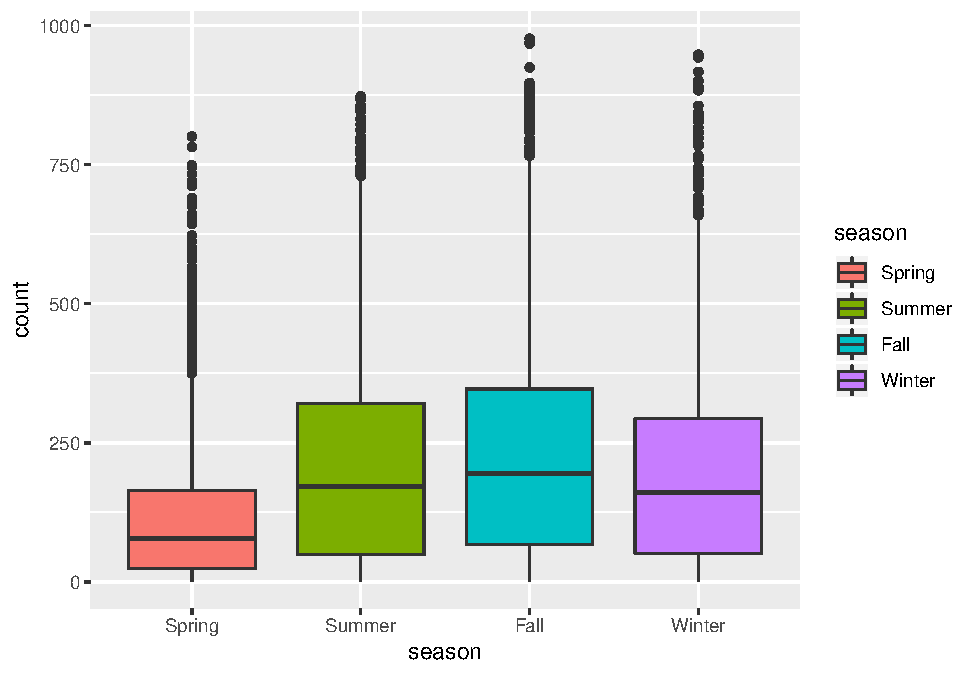
\includegraphics{BikeSharingDemand_files/figure-latex/train.mod.1.season-1.pdf}

\newpage

\hypertarget{holiday}{%
\paragraph{Holiday}\label{holiday}}

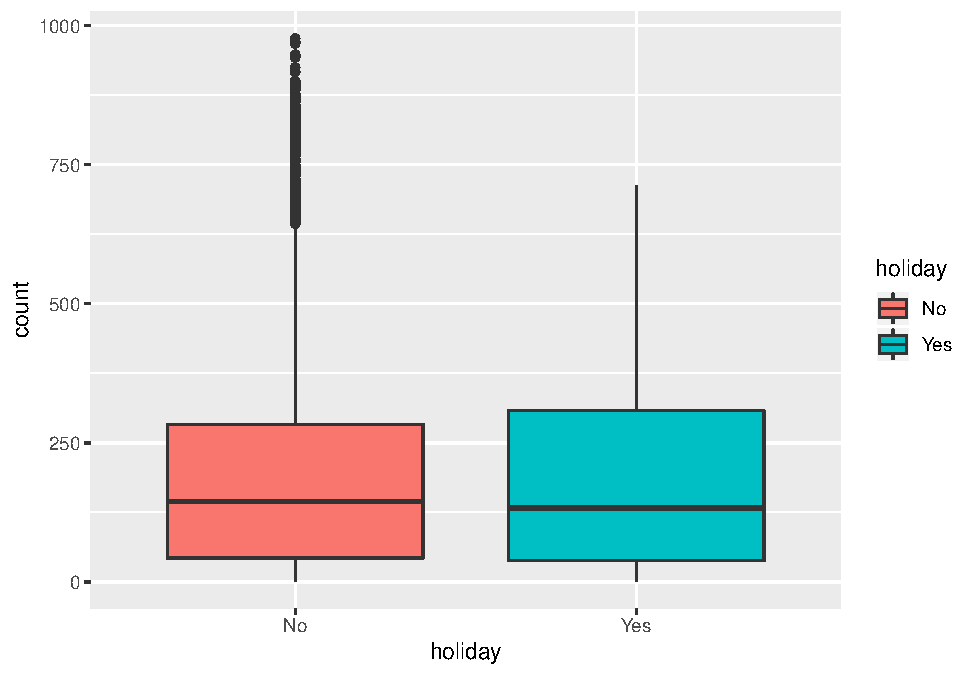
\includegraphics{BikeSharingDemand_files/figure-latex/train.mod.1.holiday-1.pdf}

\hypertarget{working-day}{%
\paragraph{Working Day}\label{working-day}}

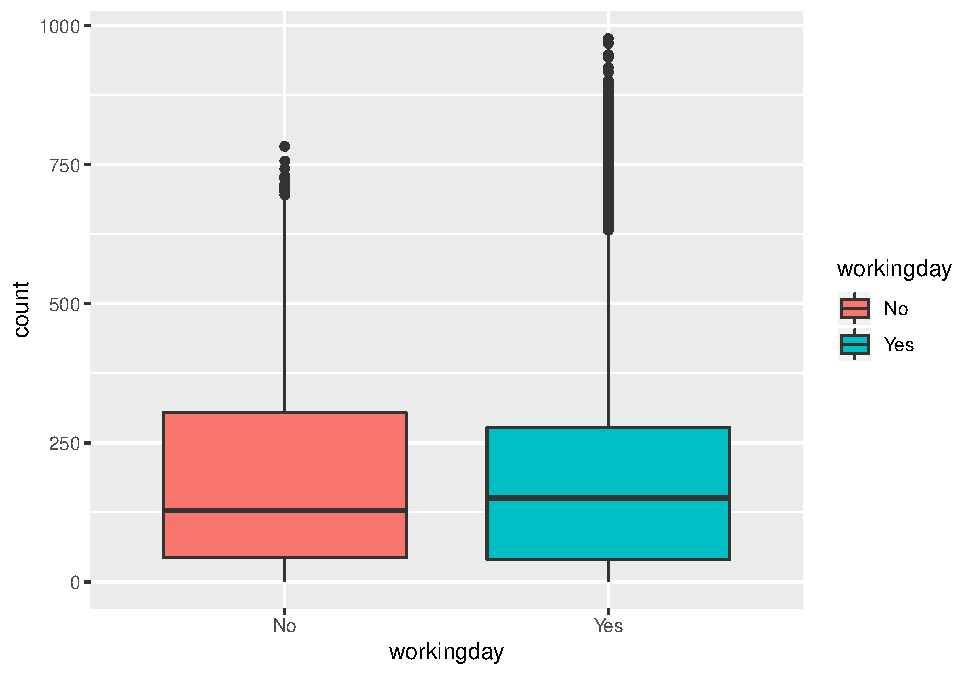
\includegraphics{BikeSharingDemand_files/figure-latex/train.mod.1.workingday-1.pdf}

\newpage

\hypertarget{weather}{%
\paragraph{Weather}\label{weather}}

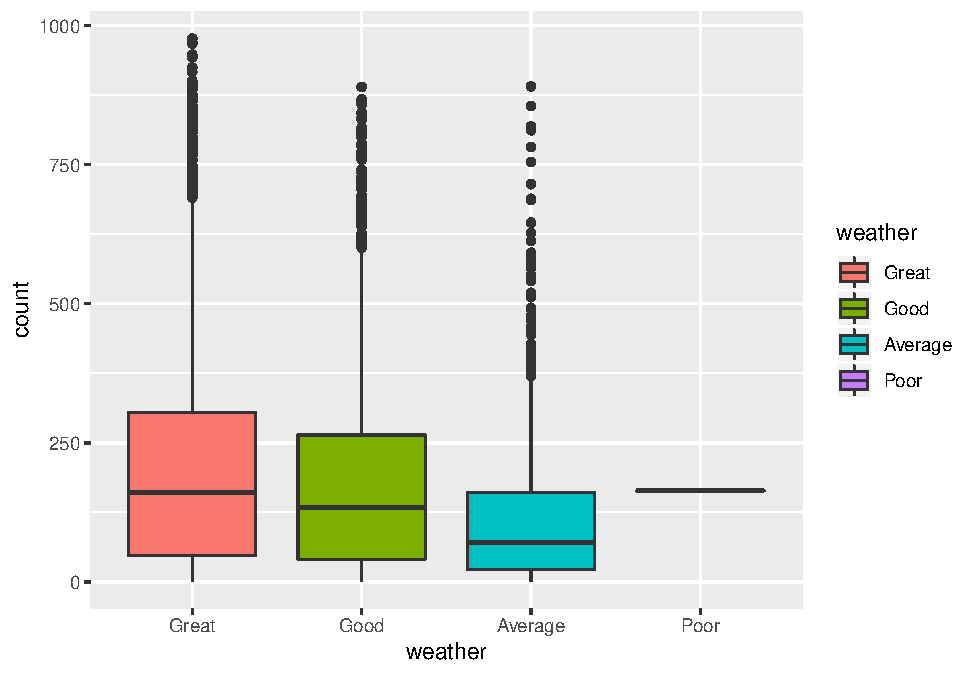
\includegraphics{BikeSharingDemand_files/figure-latex/train.mod.1.weather-1.pdf}

\newpage

\hypertarget{count-by-month}{%
\paragraph{Count by Month}\label{count-by-month}}

The datetime column was broken out into multiple factors as well so that we could visualize the components of each date and aggregate by different dimensions of the timestamp. We felt this was also necessary due to the nature of how the train/ test data sets had been pre-split. (i.e\ldots{}with the first 19 days of the month holding the only true counts to validate our models against.)

\begin{itemize}
\tightlist
\item
  Year
\item
  Month
\item
  Day
\item
  Hour
\end{itemize}

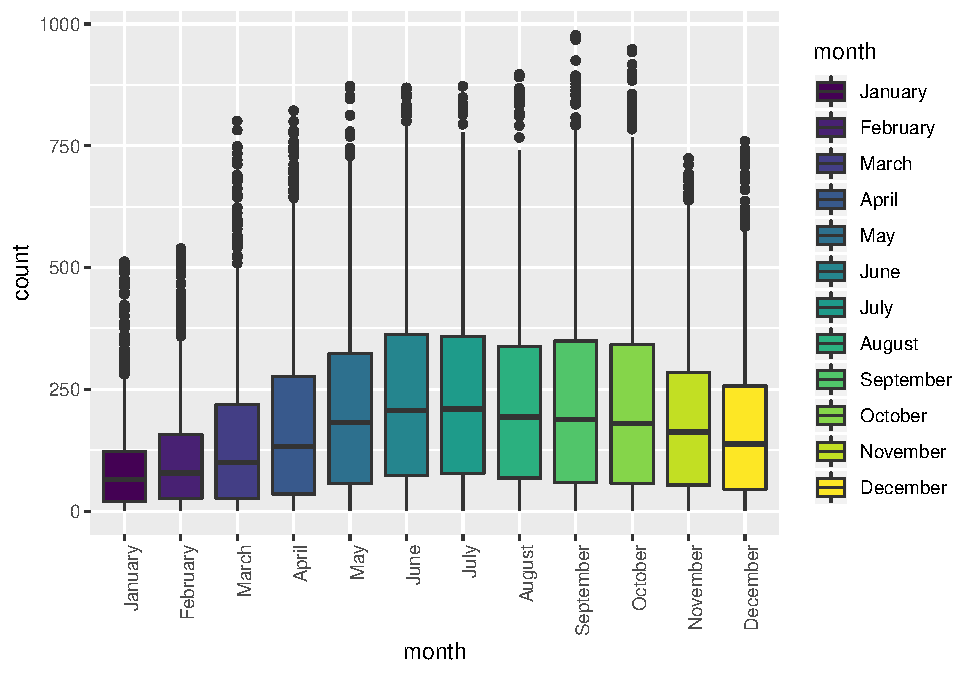
\includegraphics{BikeSharingDemand_files/figure-latex/train.mod.1.month-1.pdf}

\newpage

\hypertarget{continuous-variables}{%
\subsubsection{Continuous Variables}\label{continuous-variables}}

\hypertarget{count-by-temperature}{%
\paragraph{Count by Temperature}\label{count-by-temperature}}

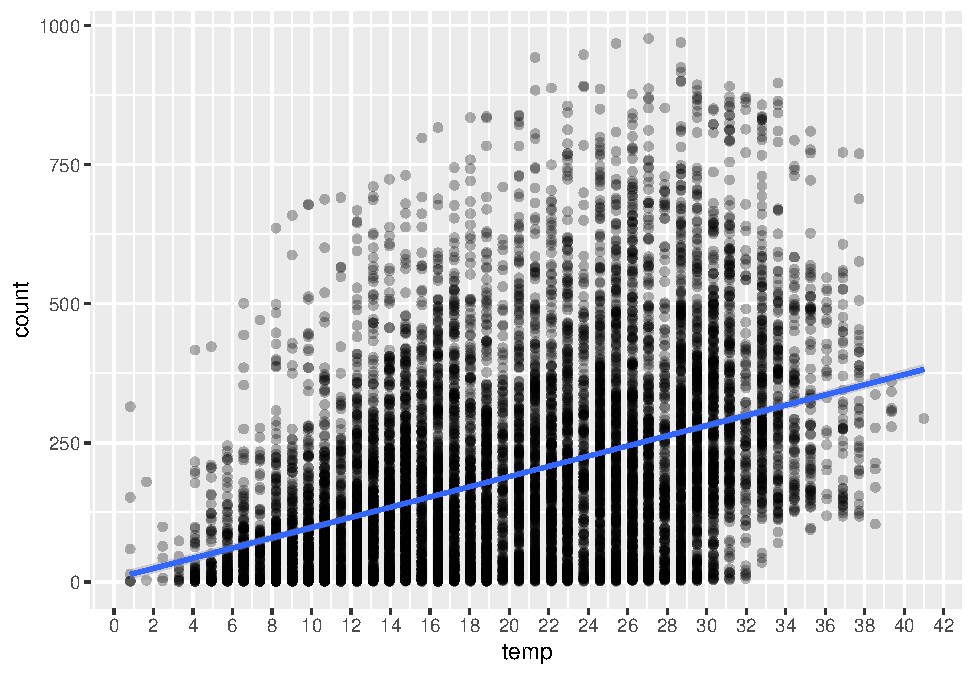
\includegraphics{BikeSharingDemand_files/figure-latex/train.mod.1.temp-1.pdf}

\newpage

\hypertarget{count-by-feels-like-temperature}{%
\paragraph{Count by ``Feels like'' Temperature}\label{count-by-feels-like-temperature}}

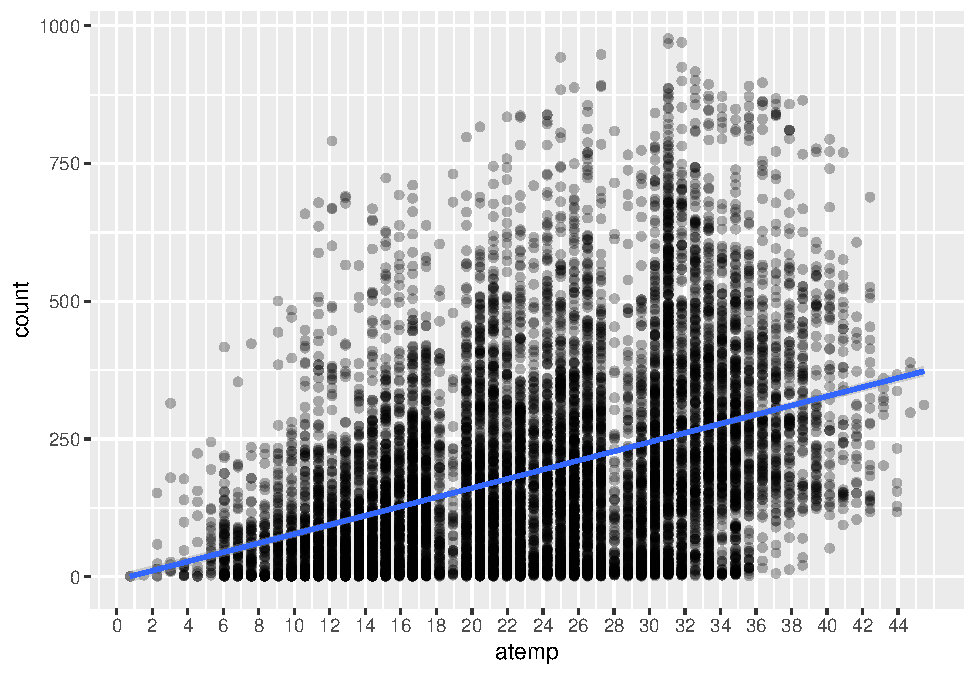
\includegraphics{BikeSharingDemand_files/figure-latex/train.mod.1.atemp-1.pdf}

\newpage

\hypertarget{count-by-wind-speed}{%
\paragraph{Count by Wind Speed}\label{count-by-wind-speed}}

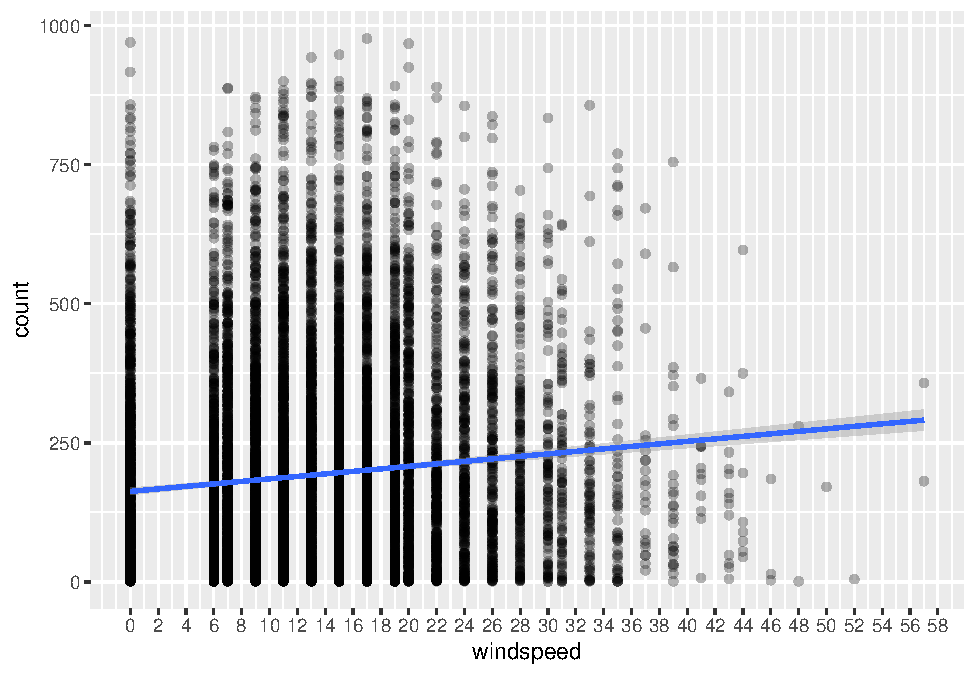
\includegraphics{BikeSharingDemand_files/figure-latex/train.mod.1.windspeed-1.pdf}

\newpage

\hypertarget{correlation-matrix}{%
\subsection{Correlation Matrix}\label{correlation-matrix}}

There are several variables with a relatively high level of covariance from the training set. The following columns should therefore be removed so as not to be picked up by any automated modelling techniques.

\begin{itemize}
\tightlist
\item
  atemp
\item
  causual
\item
  registered
\end{itemize}

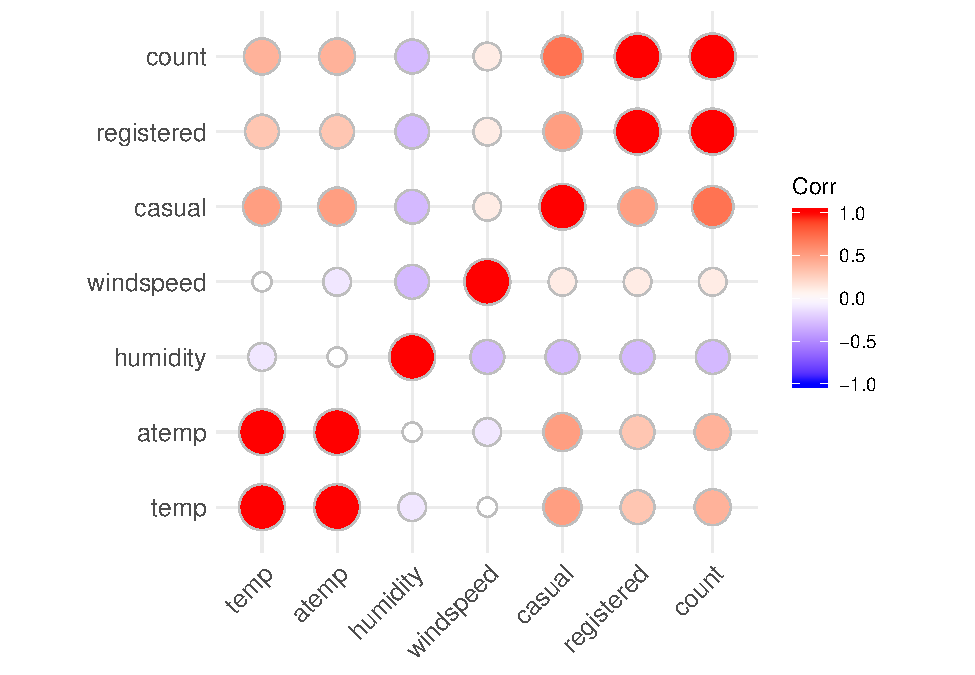
\includegraphics{BikeSharingDemand_files/figure-latex/train.mod.1.corr.matrix-1.pdf}

\newpage

\hypertarget{objective-i-analysis}{%
\section{Objective I Analysis}\label{objective-i-analysis}}

\hypertarget{question-of-interest}{%
\subsection{Question of Interest}\label{question-of-interest}}

The team be utilizing the multiple linear regression techniques we've learned up to this point in the program to predict the bike rental deman on a given date and time. The model will be evaluated on the Root Mean Squared Logarithmic Error, or RMSLE. As this data represents hourly data collected, there is an obvious time component associated with this particular competition. We wanted to gauge how effective mutiple linear regression would be when the assumption of indepdence is clearly violated.

\hypertarget{model-selection}{%
\subsection{Model Selection}\label{model-selection}}

\hypertarget{lasso}{%
\subsubsection{Lasso}\label{lasso}}

\begin{Shaded}
\begin{Highlighting}[]
\NormalTok{split.perc =}\StringTok{ }\FloatTok{.80}

\NormalTok{train.indices =}\StringTok{ }\KeywordTok{sample}\NormalTok{(}\DecValTok{1}\OperatorTok{:}\KeywordTok{dim}\NormalTok{(train.mod}\FloatTok{.1}\NormalTok{)[}\DecValTok{1}\NormalTok{],}\KeywordTok{round}\NormalTok{(split.perc }\OperatorTok{*}\StringTok{ }\KeywordTok{dim}\NormalTok{(train.mod}\FloatTok{.1}\NormalTok{)[}\DecValTok{1}\NormalTok{]))}

\NormalTok{train.mod.}\FloatTok{1.}\NormalTok{train =}\StringTok{ }\NormalTok{train.mod}\FloatTok{.1}\NormalTok{[train.indices,]}
\NormalTok{train.mod.}\FloatTok{1.}\NormalTok{test  =}\StringTok{ }\NormalTok{train.mod}\FloatTok{.1}\NormalTok{[}\OperatorTok{-}\NormalTok{train.indices,]}


\NormalTok{train.mod.}\FloatTok{1.}\NormalTok{train}\OperatorTok{$}\NormalTok{datetime <-}\StringTok{ }\OtherTok{NULL}
\NormalTok{train.mod.}\FloatTok{1.}\NormalTok{test}\OperatorTok{$}\NormalTok{datetime <-}\StringTok{ }\OtherTok{NULL}


\NormalTok{train.mod.}\FloatTok{1.}\NormalTok{train}
\end{Highlighting}
\end{Shaded}

\begin{verbatim}
## # A tibble: 8,624 x 12
##    season holiday workingday weather  temp humidity windspeed count year 
##    <fct>  <fct>   <fct>      <fct>   <dbl>    <dbl>     <dbl> <dbl> <fct>
##  1 Fall   No      Yes        Average 28.7        89     13.0   1.61 2012 
##  2 Spring No      Yes        Great   21.3        27     31.0   4.77 2011 
##  3 Fall   No      No         Great   28.7        54     11.0   6.17 2012 
##  4 Winter No      Yes        Great    9.84       75      0     2.30 2011 
##  5 Spring No      Yes        Good     8.2        34     19.0   4.16 2011 
##  6 Summer No      No         Good    28.7        48      6.00  5.48 2011 
##  7 Winter No      Yes        Great   13.9        46     15.0   6.30 2012 
##  8 Spring No      Yes        Great    9.02       51     20.0   4.04 2011 
##  9 Fall   No      Yes        Great   20.5        82      0     5.27 2012 
## 10 Fall   No      Yes        Great   30.3        70     19.0   5.19 2012 
## # ... with 8,614 more rows, and 3 more variables: month <ord>, day <fct>,
## #   hour <fct>
\end{verbatim}

\begin{Shaded}
\begin{Highlighting}[]
\NormalTok{x <-}\StringTok{ }\KeywordTok{model.matrix}\NormalTok{(count}\OperatorTok{~}\NormalTok{.,train.mod.}\FloatTok{1.}\NormalTok{train)[,}\OperatorTok{-}\DecValTok{7}\NormalTok{]}
\NormalTok{y <-}\StringTok{ }\NormalTok{train.mod.}\FloatTok{1.}\NormalTok{train}\OperatorTok{$}\NormalTok{count}

\NormalTok{grid=}\DecValTok{10}\OperatorTok{^}\KeywordTok{seq}\NormalTok{(}\DecValTok{10}\NormalTok{,}\OperatorTok{-}\DecValTok{2}\NormalTok{, }\DataTypeTok{length =}\DecValTok{100}\NormalTok{)}
\NormalTok{lasso.model <-}\StringTok{ }\KeywordTok{glmnet}\NormalTok{(x,y,}\DataTypeTok{alpha=}\DecValTok{1}\NormalTok{, }\DataTypeTok{lambda=}\NormalTok{grid)}

\NormalTok{xtest<-}\KeywordTok{model.matrix}\NormalTok{(count}\OperatorTok{~}\NormalTok{.,train.mod.}\FloatTok{1.}\NormalTok{test)[,}\OperatorTok{-}\DecValTok{7}\NormalTok{]}
\NormalTok{ytest <-}\StringTok{ }\NormalTok{train.mod.}\FloatTok{1.}\NormalTok{test}\OperatorTok{$}\NormalTok{count}


\NormalTok{cv.out=}\KeywordTok{cv.glmnet}\NormalTok{(x,y,}\DataTypeTok{alpha=}\DecValTok{1}\NormalTok{) }\CommentTok{#alpha=1 performs LASSO}
\KeywordTok{plot}\NormalTok{(cv.out)}
\end{Highlighting}
\end{Shaded}

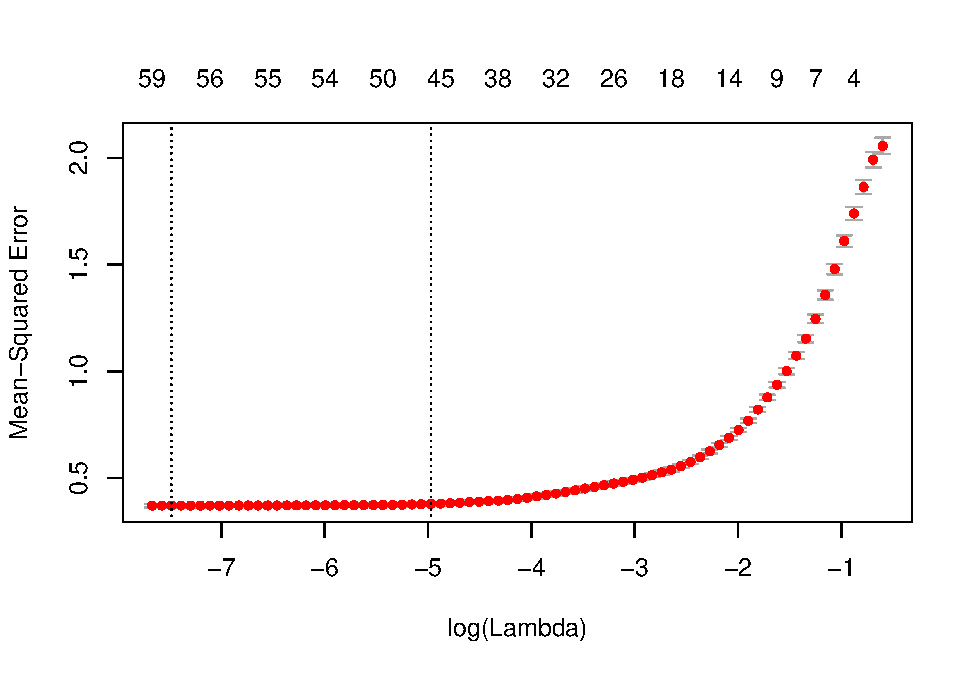
\includegraphics{BikeSharingDemand_files/figure-latex/unnamed-chunk-1-1.pdf}

\begin{Shaded}
\begin{Highlighting}[]
\NormalTok{best.lambda <-cv.out}\OperatorTok{$}\NormalTok{lambda.min  }\CommentTok{#Optimal penalty parameter.  You can make this call visually.}
\NormalTok{lasso.pred=}\KeywordTok{predict}\NormalTok{(lasso.model ,}\DataTypeTok{s=}\NormalTok{best.lambda ,}\DataTypeTok{newx=}\NormalTok{xtest)}

\NormalTok{testMSE_LASSO <-}\StringTok{ }\KeywordTok{mean}\NormalTok{((ytest}\OperatorTok{-}\NormalTok{lasso.pred)}\OperatorTok{^}\DecValTok{2}\NormalTok{)}
\NormalTok{testMSE_LASSO}
\end{Highlighting}
\end{Shaded}

\begin{verbatim}
## [1] 0.3535176
\end{verbatim}

\hypertarget{custom-variable-selection}{%
\subsubsection{Custom Variable Selection}\label{custom-variable-selection}}

We developed the best fitting model with a custom selection of variables after having accounted for those with high correlation and adding interactive terms such as month/ hour based on the seasonal nature that the box plots exhibited.

\begin{verbatim}
## Warning: not plotting observations with leverage one:
##   5555

## Warning: not plotting observations with leverage one:
##   5555
\end{verbatim}

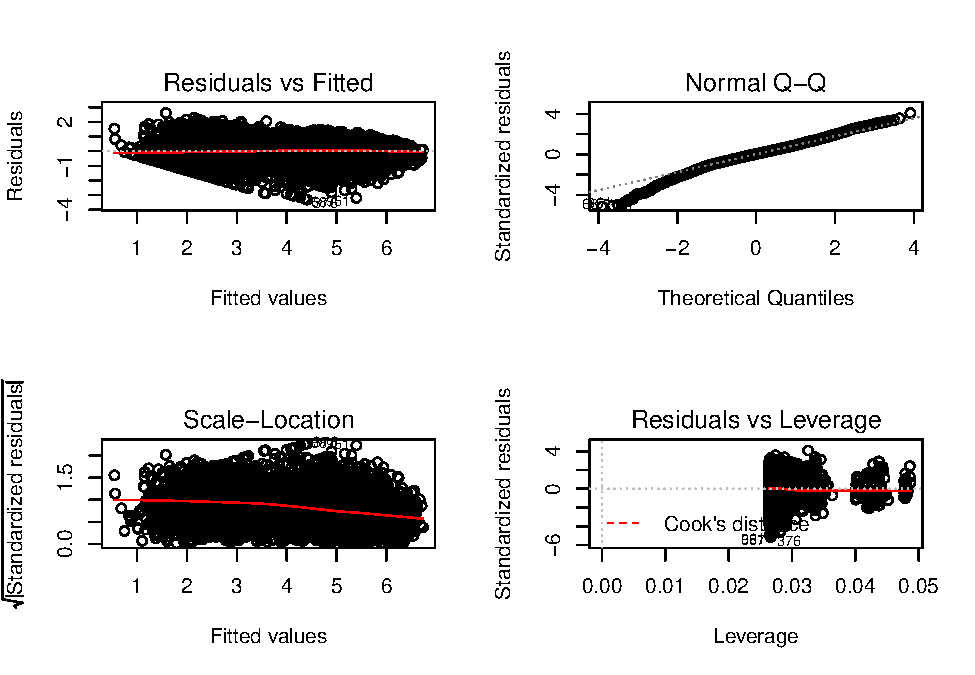
\includegraphics{BikeSharingDemand_files/figure-latex/custom-model-1.pdf} 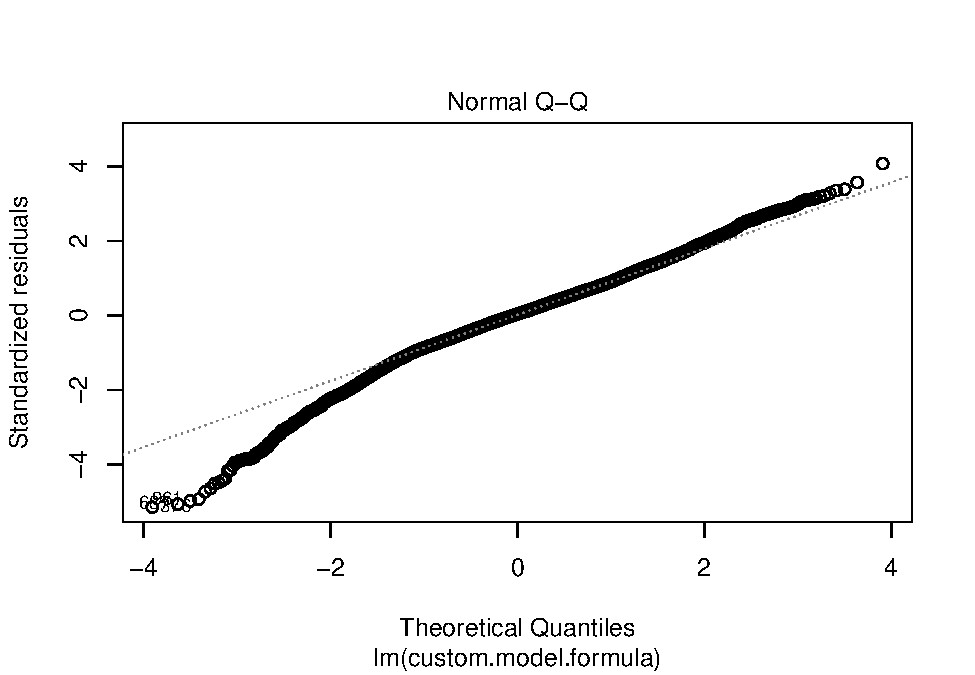
\includegraphics{BikeSharingDemand_files/figure-latex/custom-model-2.pdf}

\hypertarget{custom-rmsle}{%
\paragraph{Custom RMSLE}\label{custom-rmsle}}

\begin{verbatim}
## [1] 0.1534782
\end{verbatim}

\hypertarget{kaggle-score}{%
\paragraph{Kaggle Score}\label{kaggle-score}}

The Root Mean Squared Logarithmic Error Loss (RMSLE) for the kaggle submission was 0.67517 for our custom model. We scored better than around 24\% of all public submission for the competition with this technique.

\label{objective-one:custom-kaggle}

\begin{center}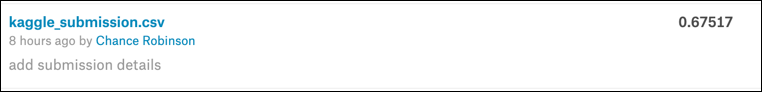
\includegraphics[width=0.9\linewidth]{./images/multiple_linear_regression_custom} \end{center}

\hypertarget{stepwise}{%
\subsubsection{Stepwise}\label{stepwise}}

\hypertarget{stepwise-rmsle}{%
\paragraph{Stepwise RMSLE}\label{stepwise-rmsle}}

The Root Mean Squared Logarithmic Error Loss calculation against the train data set.

\begin{verbatim}
## [1] 0.1469294
\end{verbatim}

\hypertarget{kaggle-score-1}{%
\paragraph{Kaggle Score}\label{kaggle-score-1}}

The Root Mean Squared Logarithmic Error Loss (RMSLE) for the kaggle submission was 0.64765 for our stepwise model. We scored better than around 24\% of all public submission for the competition with this technique, which was almost identical to that of the custom model with an interaction.

\label{objective-one:stepwise-kaggle}

\begin{center}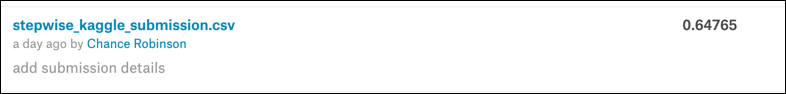
\includegraphics[width=0.9\linewidth]{./images/multiple_linear_regression_stepwise} \end{center}

\newpage

\hypertarget{model-assumptions-assessment}{%
\subsection{Model Assumptions Assessment}\label{model-assumptions-assessment}}

\begin{itemize}
\tightlist
\item
  The response variable is linear
\item
  The data is normally distributed
\item
  Independence
\end{itemize}

\hypertarget{comparing-competing-models}{%
\subsection{Comparing Competing Models}\label{comparing-competing-models}}

\newpage

\hypertarget{parameters}{%
\subsection{Parameters}\label{parameters}}

\protect\hyperlink{parameters}{Parameters}

\hypertarget{model-interpretation}{%
\subsection{Model Interpretation}\label{model-interpretation}}

\protect\hyperlink{model-interpretation}{Model Interpretation}

\hypertarget{conclusion}{%
\subsection{Conclusion}\label{conclusion}}

\protect\hyperlink{conclusion-1}{Conclusion}

\newpage

\hypertarget{objective-ii-analysis}{%
\section{Objective II Analysis}\label{objective-ii-analysis}}

\hypertarget{question-of-interest-1}{%
\subsection{Question of Interest}\label{question-of-interest-1}}

As the independence assumption from Objective I appears to have been violated, the team wanted to apply the time series analysis techniques we've learned up to this point in the MSDS program in an attempt to address. The primary goal was to compare and contrast the performance of auto arima models versus those that we modeled on our own.

Additionally, we wanted to compare the Kaggle submission to that from Objective I to see if our predictions were better or worse than from the prior objective.

\hypertarget{data-preperation}{%
\subsection{Data Preperation}\label{data-preperation}}

As the data had been pre-split monthly, we needed to make our predictions from the 20th of each month and on for each year of recorded bike rentals. (2011 and 2012) The approach has been summarized with the steps below.

\begin{enumerate}
\def\labelenumi{\arabic{enumi}.}
\item
  Log the response variable
\item
  Loop through years
\item
  Loop through months
\item
  Fit AR model
\item
  Forcast x number of observations based on the number of rows from test dataframe and impute the count from the time series forecast
\end{enumerate}

\newpage

\hypertarget{comparing-competing-models-1}{%
\subsection{Comparing Competing Models}\label{comparing-competing-models-1}}

\hypertarget{auto-arima}{%
\subsubsection{Auto Arima}\label{auto-arima}}

\begin{verbatim}
## 
##  Ljung-Box test
## 
## data:  Residuals from ARIMA(4,0,4) with non-zero mean
## Q* = 10.049, df = 3, p-value = 0.01816
## 
## Model df: 9.   Total lags used: 12
\end{verbatim}

\begin{figure}[htbp]

{\centering 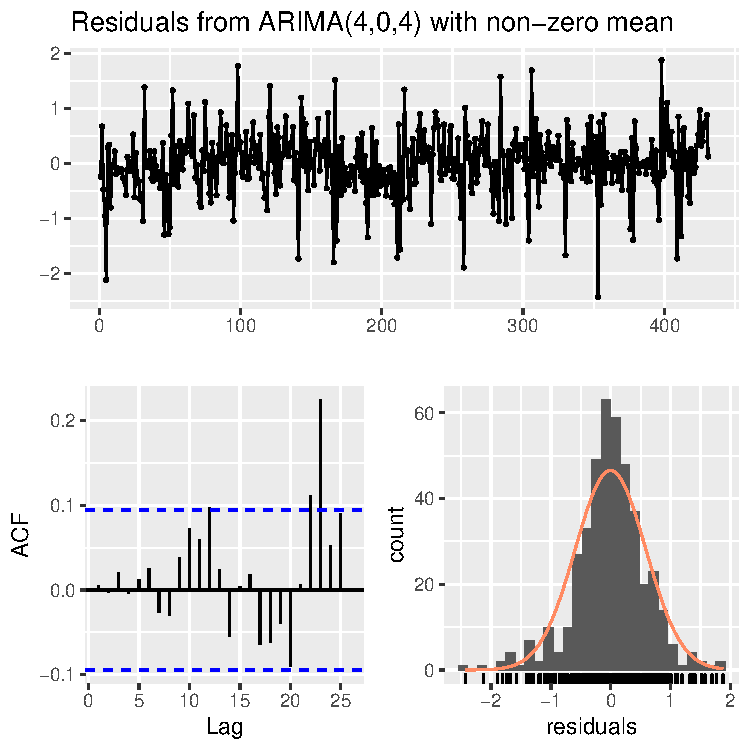
\includegraphics[width=0.45\linewidth]{BikeSharingDemand_files/figure-latex/auto-arima-plot-1-1} 

}

\caption{Auto Arima Residual Plots}\label{fig:auto-arima-plot-1}
\end{figure}

\begin{figure}[htbp]

{\centering 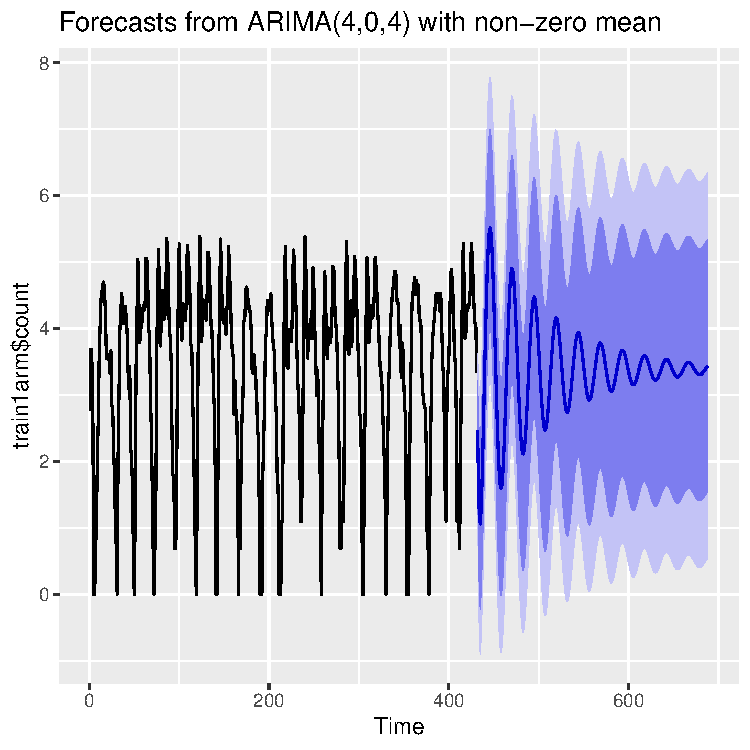
\includegraphics[width=0.45\linewidth]{BikeSharingDemand_files/figure-latex/auto-arima-plot-2-1} 

}

\caption{Auto Arima Forecasts}\label{fig:auto-arima-plot-2}
\end{figure}

\newpage

\hypertarget{auto-regression}{%
\subsubsection{Auto Regression}\label{auto-regression}}

\begin{verbatim}
## 
##  Ljung-Box test
## 
## data:  Residuals from ARIMA(25,0,0) with non-zero mean
## Q* = 11.131, df = 3, p-value = 0.01104
## 
## Model df: 26.   Total lags used: 29
\end{verbatim}

\begin{figure}[htbp]

{\centering 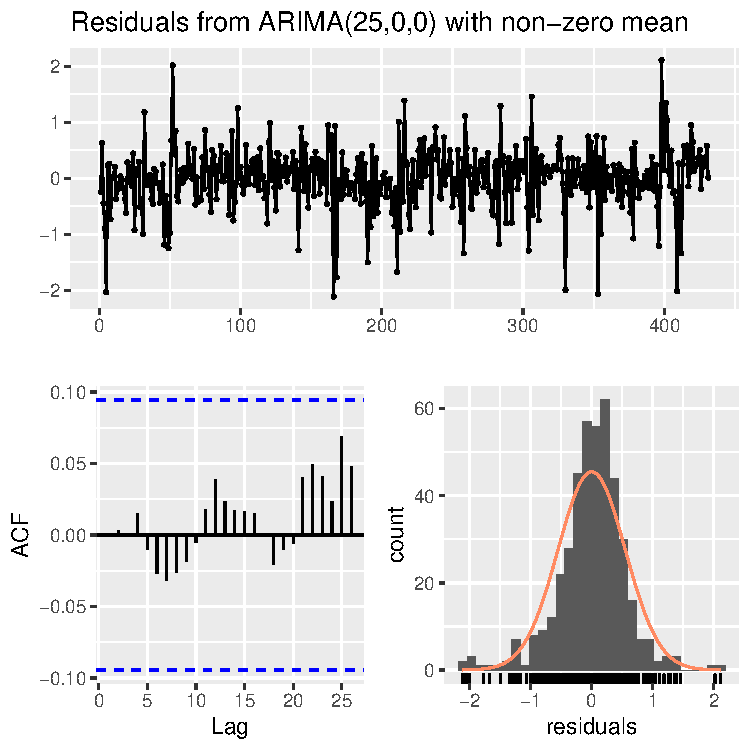
\includegraphics[width=0.45\linewidth]{BikeSharingDemand_files/figure-latex/arima-25-plot-1-1} 

}

\caption{Arima (25) Residual Plots}\label{fig:arima-25-plot-1}
\end{figure}

\begin{figure}[htbp]

{\centering 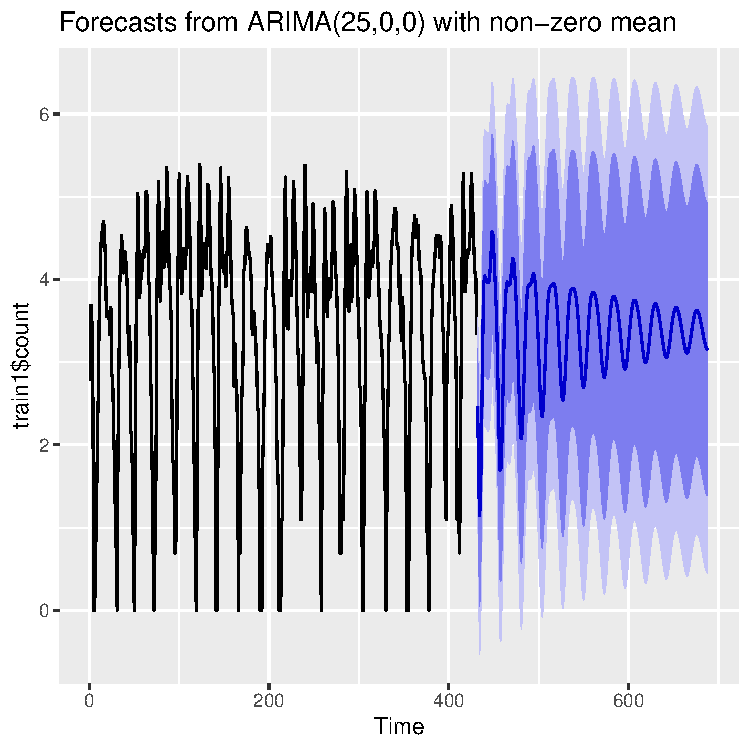
\includegraphics[width=0.45\linewidth]{BikeSharingDemand_files/figure-latex/arima-25-plot-2-1} 

}

\caption{Arima (25) Forecasts}\label{fig:arima-25-plot-2}
\end{figure}

\newpage

\hypertarget{accuracy-metrics}{%
\subsubsection{Accuracy Metrics}\label{accuracy-metrics}}

The accuracy metrics appear to go in favor of the AR25 model.

\begin{table}[H]
\centering
\begin{tabular}{lrrr}
\toprule
Model & RMSLE & AIC & Variance\\
\midrule
ARIMA & 0.2418941 & 791.5698 & 0.3541476\\
AR25 & 0.2265693 & 768.3810 & 0.3025818\\
\bottomrule
\end{tabular}
\end{table}

\newpage

\hypertarget{kaggle-score-2}{%
\paragraph{Kaggle Score}\label{kaggle-score-2}}

The Root Mean Squared Logarithmic Error Loss (RMSLE) for the kaggle submission was 1.01847 for our AR25 model. We scored better than only 14.48\% of all public submission for the competition which was considerably worse than our score from both of the multiple linear regression models above.

\label{objective-two:ar25-kaggle}

\begin{center}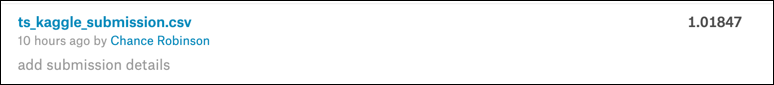
\includegraphics[width=0.9\linewidth]{./images/time_series_ar25} \end{center}

\hypertarget{model-assumption-assessment}{%
\subsection{Model Assumption Assessment}\label{model-assumption-assessment}}

Both the ARIMA and AR 25 models showed a constant mean and variance for the timespan of the observations. The auto-correlations however were noticably better for the AR 25 graph. The error terms were also slightly improved which is the reason we elected to not go with the automated selection approach.

\begin{itemize}
\tightlist
\item
  Constant Mean
\item
  Constant Variance
\item
  Constant auto-correlations
\end{itemize}

\hypertarget{conclusion-1}{%
\subsection{Conclusion}\label{conclusion-1}}

Although the data set was found to be serially correlated, ultimately applying time series techniques was not sufficient to improve our RMSLE above and beyond the multiple linear regression techniques from objective one. Again, this likely had more to due with the fact that we were attempting to predict future observations 10 plus days in advance on a monthly basis. And with the seasonal nature of our hourly observations, the accuracy of the preduction became less accurate over time and showed a regression to the mean after only a few days worth of predictions. The immediate observations however, within 24 to 48 hours, visually at least showed much better predictive trends.

\newpage

\hypertarget{appendix}{%
\section{Appendix}\label{appendix}}

\hypertarget{code}{%
\subsection{Code}\label{code}}

\hypertarget{r-code-for-objective-i}{%
\subsubsection{R Code For Objective I}\label{r-code-for-objective-i}}

\newpage

\hypertarget{r-code-for-objective-ii}{%
\subsubsection{R Code For Objective II}\label{r-code-for-objective-ii}}

\begin{Shaded}
\begin{Highlighting}[]
\CommentTok{### Library Imports}

\KeywordTok{library}\NormalTok{(tidyverse)}
\CommentTok{# Date manipulation}
\KeywordTok{library}\NormalTok{(lubridate)}
\CommentTok{# RMLSE}
\KeywordTok{library}\NormalTok{(MLmetrics)}
\CommentTok{# Time Series Analysis}
\KeywordTok{library}\NormalTok{(tseries)}
\KeywordTok{library}\NormalTok{(forecast)}


\CommentTok{### Load the csv data}
\NormalTok{train <-}\StringTok{ }\KeywordTok{read_csv}\NormalTok{(}\StringTok{'../../../data/train.csv'}\NormalTok{)}
\NormalTok{test <-}\StringTok{ }\KeywordTok{read_csv}\NormalTok{(}\StringTok{'../../../data/test.csv'}\NormalTok{)}


\CommentTok{### Categorical Factors}
\NormalTok{train}\OperatorTok{$}\NormalTok{season <-}\StringTok{ }\KeywordTok{factor}\NormalTok{(train}\OperatorTok{$}\NormalTok{season, }\DataTypeTok{labels =} \KeywordTok{c}\NormalTok{(}\StringTok{"Spring"}\NormalTok{, }\StringTok{"Summer"}\NormalTok{, }\StringTok{"Fall"}\NormalTok{, }\StringTok{"Winter"}\NormalTok{))}
\NormalTok{test}\OperatorTok{$}\NormalTok{season <-}\StringTok{ }\KeywordTok{factor}\NormalTok{(test}\OperatorTok{$}\NormalTok{season, }\DataTypeTok{labels =} \KeywordTok{c}\NormalTok{(}\StringTok{"Spring"}\NormalTok{, }\StringTok{"Summer"}\NormalTok{, }\StringTok{"Fall"}\NormalTok{, }\StringTok{"Winter"}\NormalTok{))}

\KeywordTok{table}\NormalTok{(train}\OperatorTok{$}\NormalTok{season)}

\NormalTok{train}\OperatorTok{$}\NormalTok{holiday <-}\StringTok{ }\KeywordTok{factor}\NormalTok{(train}\OperatorTok{$}\NormalTok{holiday, }\DataTypeTok{labels =} \KeywordTok{c}\NormalTok{(}\StringTok{"No"}\NormalTok{, }\StringTok{"Yes"}\NormalTok{))}
\NormalTok{test}\OperatorTok{$}\NormalTok{holiday <-}\StringTok{ }\KeywordTok{factor}\NormalTok{(test}\OperatorTok{$}\NormalTok{holiday, }\DataTypeTok{labels =} \KeywordTok{c}\NormalTok{(}\StringTok{"No"}\NormalTok{, }\StringTok{"Yes"}\NormalTok{))}

\KeywordTok{table}\NormalTok{(train}\OperatorTok{$}\NormalTok{holiday)}

\NormalTok{train}\OperatorTok{$}\NormalTok{workingday <-}\StringTok{ }\KeywordTok{factor}\NormalTok{(train}\OperatorTok{$}\NormalTok{workingday, }\DataTypeTok{labels =} \KeywordTok{c}\NormalTok{(}\StringTok{"No"}\NormalTok{, }\StringTok{"Yes"}\NormalTok{))}
\NormalTok{test}\OperatorTok{$}\NormalTok{workingday <-}\StringTok{ }\KeywordTok{factor}\NormalTok{(test}\OperatorTok{$}\NormalTok{workingday, }\DataTypeTok{labels =} \KeywordTok{c}\NormalTok{(}\StringTok{"No"}\NormalTok{, }\StringTok{"Yes"}\NormalTok{))}

\KeywordTok{table}\NormalTok{(train}\OperatorTok{$}\NormalTok{workingday)}

\NormalTok{train}\OperatorTok{$}\NormalTok{weather <-}\StringTok{ }\KeywordTok{factor}\NormalTok{(train}\OperatorTok{$}\NormalTok{weather, }\DataTypeTok{labels =} \KeywordTok{c}\NormalTok{(}\StringTok{"Great"}\NormalTok{, }\StringTok{"Good"}\NormalTok{, }\StringTok{"Average"}\NormalTok{, }\StringTok{"Poor"}\NormalTok{))}
\NormalTok{test}\OperatorTok{$}\NormalTok{weather <-}\StringTok{ }\KeywordTok{factor}\NormalTok{(test}\OperatorTok{$}\NormalTok{weather, }\DataTypeTok{labels =} \KeywordTok{c}\NormalTok{(}\StringTok{"Great"}\NormalTok{, }\StringTok{"Good"}\NormalTok{, }\StringTok{"Average"}\NormalTok{, }\StringTok{"Poor"}\NormalTok{))}

\KeywordTok{table}\NormalTok{(train}\OperatorTok{$}\NormalTok{weather)}


\CommentTok{### Split Date-Time}
\NormalTok{train <-}\StringTok{ }\NormalTok{train }\OperatorTok
\StringTok{  }\KeywordTok{mutate}\NormalTok{(}\DataTypeTok{year =} \KeywordTok{as.factor}\NormalTok{(}\KeywordTok{format}\NormalTok{(datetime, }\DataTypeTok{format =} \StringTok{"%Y"}\NormalTok{)), }
         \DataTypeTok{month =} \KeywordTok{as.numeric}\NormalTok{(}\KeywordTok{format}\NormalTok{(datetime, }\DataTypeTok{format =} \StringTok{"%m"}\NormalTok{)), }
         \DataTypeTok{day =} \KeywordTok{as.factor}\NormalTok{(}\KeywordTok{format}\NormalTok{(datetime, }\DataTypeTok{format =} \StringTok{"%d"}\NormalTok{)),}
         \DataTypeTok{hour =} \KeywordTok{as.factor}\NormalTok{(}\KeywordTok{format}\NormalTok{(datetime, }\DataTypeTok{format =} \StringTok{"%H"}\NormalTok{)))}

\NormalTok{test <-}\StringTok{ }\NormalTok{test }\OperatorTok
\StringTok{  }\KeywordTok{mutate}\NormalTok{(}\DataTypeTok{year =} \KeywordTok{as.factor}\NormalTok{(}\KeywordTok{format}\NormalTok{(datetime, }\DataTypeTok{format =} \StringTok{"%Y"}\NormalTok{)), }
         \DataTypeTok{month =} \KeywordTok{as.numeric}\NormalTok{(}\KeywordTok{format}\NormalTok{(datetime, }\DataTypeTok{format =} \StringTok{"%m"}\NormalTok{)), }
         \DataTypeTok{day =} \KeywordTok{as.factor}\NormalTok{(}\KeywordTok{format}\NormalTok{(datetime, }\DataTypeTok{format =} \StringTok{"%d"}\NormalTok{)),}
         \DataTypeTok{hour =} \KeywordTok{as.factor}\NormalTok{(}\KeywordTok{format}\NormalTok{(datetime, }\DataTypeTok{format =} \StringTok{"%H"}\NormalTok{)))}


\CommentTok{### Convert months to ordinal factor}
\NormalTok{train}\OperatorTok{$}\NormalTok{month <-}\KeywordTok{month}\NormalTok{(train}\OperatorTok{$}\NormalTok{datetime, }\DataTypeTok{label =} \OtherTok{TRUE}\NormalTok{, }\DataTypeTok{abbr =} \OtherTok{FALSE}\NormalTok{)}
\NormalTok{test}\OperatorTok{$}\NormalTok{month <-}\KeywordTok{month}\NormalTok{(test}\OperatorTok{$}\NormalTok{datetime, }\DataTypeTok{label =} \OtherTok{TRUE}\NormalTok{, }\DataTypeTok{abbr =} \OtherTok{FALSE}\NormalTok{)}


\CommentTok{## 2011}

\CommentTok{### January}

\CommentTok{#### Auto Arima}

\NormalTok{train1arm <-}\StringTok{ }\NormalTok{train }\OperatorTok
\StringTok{  }\KeywordTok{filter}\NormalTok{(year }\OperatorTok{==}\StringTok{ '2011'} \OperatorTok{&}\StringTok{ }\NormalTok{month }\OperatorTok{==}\StringTok{ 'January'}\NormalTok{) }\OperatorTok
\StringTok{  }\KeywordTok{select}\NormalTok{(datetime, count)}

\NormalTok{test1arm <-}\StringTok{ }\NormalTok{test }\OperatorTok
\StringTok{  }\KeywordTok{filter}\NormalTok{(year }\OperatorTok{==}\StringTok{ '2011'} \OperatorTok{&}\StringTok{ }\NormalTok{month }\OperatorTok{==}\StringTok{ 'January'}\NormalTok{) }\OperatorTok
\StringTok{  }\KeywordTok{mutate}\NormalTok{(}\DataTypeTok{count =} \OtherTok{NA}\NormalTok{) }\OperatorTok
\StringTok{  }\KeywordTok{select}\NormalTok{(datetime, count)}


\CommentTok{### Log the response variable}
\NormalTok{train1arm}\OperatorTok{$}\NormalTok{count =}\StringTok{ }\KeywordTok{log}\NormalTok{(train1arm}\OperatorTok{$}\NormalTok{count)}


\NormalTok{autoarm <-}\StringTok{ }\KeywordTok{auto.arima}\NormalTok{(train1arm}\OperatorTok{$}\NormalTok{count, }\DataTypeTok{D=}\DecValTok{1}\NormalTok{)}


\NormalTok{number =}\StringTok{ }\KeywordTok{nrow}\NormalTok{(test1arm)}

\KeywordTok{acf}\NormalTok{(autoarm}\OperatorTok{$}\NormalTok{residuals)}
\KeywordTok{pacf}\NormalTok{(autoarm}\OperatorTok{$}\NormalTok{residuals)}

\KeywordTok{checkresiduals}\NormalTok{(autoarm)}

\NormalTok{fcst <-}\StringTok{ }\KeywordTok{forecast}\NormalTok{(autoarm, }\DataTypeTok{h=}\NormalTok{number)}

\KeywordTok{autoplot}\NormalTok{(fcst)}

\CommentTok{# point estimate (mean)}
\NormalTok{test1arm}\OperatorTok{$}\NormalTok{count <-}\StringTok{ }\NormalTok{fcst}\OperatorTok{$}\NormalTok{mean}

\KeywordTok{RMSLE}\NormalTok{(}\DataTypeTok{y_pred =}\NormalTok{ fcst}\OperatorTok{$}\NormalTok{fitted, }\DataTypeTok{y_true =}\NormalTok{ train1arm}\OperatorTok{$}\NormalTok{count)}

\KeywordTok{summary}\NormalTok{(autoarm)}


\CommentTok{#### AR 25}

\NormalTok{train1 <-}\StringTok{ }\NormalTok{train }\OperatorTok
\StringTok{  }\KeywordTok{filter}\NormalTok{(year }\OperatorTok{==}\StringTok{ '2011'} \OperatorTok{&}\StringTok{ }\NormalTok{month }\OperatorTok{==}\StringTok{ 'January'}\NormalTok{) }\OperatorTok
\StringTok{  }\KeywordTok{select}\NormalTok{(datetime, count)}

\NormalTok{test1 <-}\StringTok{ }\NormalTok{test }\OperatorTok
\StringTok{  }\KeywordTok{filter}\NormalTok{(year }\OperatorTok{==}\StringTok{ '2011'} \OperatorTok{&}\StringTok{ }\NormalTok{month }\OperatorTok{==}\StringTok{ 'January'}\NormalTok{) }\OperatorTok
\StringTok{  }\KeywordTok{mutate}\NormalTok{(}\DataTypeTok{count =} \OtherTok{NA}\NormalTok{) }\OperatorTok
\StringTok{  }\KeywordTok{select}\NormalTok{(datetime, count)}


\CommentTok{### Log the response variable}
\NormalTok{train1}\OperatorTok{$}\NormalTok{count =}\StringTok{ }\KeywordTok{log}\NormalTok{(train1}\OperatorTok{$}\NormalTok{count)}


\NormalTok{AR25 <-}\StringTok{ }\KeywordTok{arima}\NormalTok{(train1}\OperatorTok{$}\NormalTok{count,}\DataTypeTok{order=}\KeywordTok{c}\NormalTok{(}\DecValTok{25}\NormalTok{,}\DecValTok{0}\NormalTok{,}\DecValTok{0}\NormalTok{))}

\NormalTok{number =}\StringTok{ }\KeywordTok{nrow}\NormalTok{(test1)}

\KeywordTok{acf}\NormalTok{(AR25}\OperatorTok{$}\NormalTok{residuals)}
\KeywordTok{pacf}\NormalTok{(AR25}\OperatorTok{$}\NormalTok{residuals)}

\KeywordTok{checkresiduals}\NormalTok{(AR25)}

\NormalTok{fcst <-}\StringTok{ }\KeywordTok{forecast}\NormalTok{(AR25, }\DataTypeTok{h=}\NormalTok{number)}

\KeywordTok{autoplot}\NormalTok{(fcst)}

\CommentTok{# point estimate (mean)}
\NormalTok{test1}\OperatorTok{$}\NormalTok{count <-}\StringTok{ }\NormalTok{fcst}\OperatorTok{$}\NormalTok{mean}


\KeywordTok{RMSLE}\NormalTok{(}\DataTypeTok{y_pred =}\NormalTok{ fcst}\OperatorTok{$}\NormalTok{fitted, }\DataTypeTok{y_true =}\NormalTok{ train1}\OperatorTok{$}\NormalTok{count)}
\KeywordTok{summary}\NormalTok{(AR25)}


\CommentTok{#}
\CommentTok{#}
\CommentTok{#}

\CommentTok{## 2012}

\CommentTok{### December}

\NormalTok{train24 <-}\StringTok{ }\NormalTok{train }\OperatorTok
\StringTok{  }\KeywordTok{filter}\NormalTok{(year }\OperatorTok{==}\StringTok{ '2012'} \OperatorTok{&}\StringTok{ }\NormalTok{month }\OperatorTok{==}\StringTok{ 'December'}\NormalTok{) }\OperatorTok
\StringTok{  }\KeywordTok{select}\NormalTok{(datetime, count)}

\NormalTok{test24 <-}\StringTok{ }\NormalTok{test }\OperatorTok
\StringTok{  }\KeywordTok{filter}\NormalTok{(year }\OperatorTok{==}\StringTok{ '2012'} \OperatorTok{&}\StringTok{ }\NormalTok{month }\OperatorTok{==}\StringTok{ 'December'}\NormalTok{) }\OperatorTok
\StringTok{  }\KeywordTok{mutate}\NormalTok{(}\DataTypeTok{count =} \OtherTok{NA}\NormalTok{) }\OperatorTok
\StringTok{  }\KeywordTok{select}\NormalTok{(datetime, count)}


\CommentTok{### Log the response variable}
\NormalTok{train24}\OperatorTok{$}\NormalTok{count =}\StringTok{ }\KeywordTok{log}\NormalTok{(train24}\OperatorTok{$}\NormalTok{count)}


\NormalTok{AR25 <-}\StringTok{ }\KeywordTok{arima}\NormalTok{(train24}\OperatorTok{$}\NormalTok{count,}\DataTypeTok{order=}\KeywordTok{c}\NormalTok{(}\DecValTok{25}\NormalTok{,}\DecValTok{0}\NormalTok{,}\DecValTok{0}\NormalTok{))}

\NormalTok{number =}\StringTok{ }\KeywordTok{nrow}\NormalTok{(test24)}

\KeywordTok{acf}\NormalTok{(AR25}\OperatorTok{$}\NormalTok{residuals)}
\KeywordTok{pacf}\NormalTok{(AR25}\OperatorTok{$}\NormalTok{residuals)}

\KeywordTok{checkresiduals}\NormalTok{(AR25)}

\NormalTok{fcst <-}\StringTok{ }\KeywordTok{forecast}\NormalTok{(AR25, }\DataTypeTok{h=}\NormalTok{number)}

\KeywordTok{autoplot}\NormalTok{(fcst)}

\CommentTok{# point estimate (mean)}
\NormalTok{test24}\OperatorTok{$}\NormalTok{count <-}\StringTok{ }\NormalTok{fcst}\OperatorTok{$}\NormalTok{mean}


\KeywordTok{RMSLE}\NormalTok{(}\DataTypeTok{y_pred =}\NormalTok{ fcst}\OperatorTok{$}\NormalTok{fitted, }\DataTypeTok{y_true =}\NormalTok{ train24}\OperatorTok{$}\NormalTok{count)}

\KeywordTok{summary}\NormalTok{(AR25)}


\CommentTok{### Combine all of the individual data frames}

\NormalTok{combined <-}\StringTok{ }\KeywordTok{data.frame}\NormalTok{(}\DataTypeTok{datetime=}\KeywordTok{character}\NormalTok{(),}
                 \DataTypeTok{count=}\KeywordTok{double}\NormalTok{(), }
                 \DataTypeTok{stringsAsFactors=}\OtherTok{FALSE}\NormalTok{) }



\NormalTok{combined <-}\StringTok{ }\KeywordTok{bind_rows}\NormalTok{(test1, test2, test3, test4, test5, }
\NormalTok{                      test6, test7, test8, test9, test10, }
\NormalTok{                      test11, test12,test13, test14, test15, }
\NormalTok{                      test16, test17, test18, test19, test20, }
\NormalTok{                      test21, test22, test23, test24)}


\NormalTok{combined <-}\StringTok{ }\NormalTok{combined }\OperatorTok
\StringTok{  }\KeywordTok{mutate}\NormalTok{(}\DataTypeTok{count =} \KeywordTok{round}\NormalTok{(}\KeywordTok{exp}\NormalTok{(count)))}


\CommentTok{# combined}
\CommentTok{# write.csv(combined, file = "./ts_kaggle_submission.csv", row.names = F)}
\end{Highlighting}
\end{Shaded}

\newpage

\renewcommand\refname{References}
\bibliography{references.bib}


\end{document}
